%------------------------------------------------------------------------------
% Beginning of journal.tex
%------------------------------------------------------------------------------
%
% AMS-LaTeX version 2 sample file for journals, based on amsart.cls.
%
%        ***     DO NOT USE THIS FILE AS A STARTER.      ***
%        ***  USE THE JOURNAL-SPECIFIC *.TEMPLATE FILE.  ***
%
% Replace amsart by the documentclass for the target journal, e.g., tran-l.
%
\documentclass{amsart}

%     If your article includes graphics, uncomment this command.
\usepackage{graphicx}
\usepackage{amsmath}
\newtheorem{theorem}{Theorem}[section]
\newtheorem{lemma}[theorem]{Lemma}

\theoremstyle{definition}
\newtheorem{definition}[theorem]{Definition}
\newtheorem{example}[theorem]{Example}
\newtheorem{xca}[theorem]{Exercise}

\theoremstyle{remark}
\newtheorem{remark}[theorem]{Remark}

\numberwithin{equation}{section}

%    Absolute value notation
\newcommand{\abs}[1]{\lvert#1\rvert}

%    Blank box placeholder for figures (to avoid requiring any
%    particular graphics capabilities for printing this document).
\newcommand{\blankbox}[2]{%
  \parbox{\columnwidth}{\centering
%    Set fboxsep to 0 so that the actual size of the box will match the
%    given measurements more closely.
    \setlength{\fboxsep}{0pt}%
    \fbox{\raisebox{0pt}[#2]{\hspace{#1}}}%
  }%
}

\begin{document}

\title{COMP 2804 - Assignment 1}
\author{Seena Rowhani}

%    General info

\date{Due: January 29th 2015}

\dedicatory{Micheal Smid}

\maketitle




\section*{QUESTION 1}
\subsection*{Assume there are $n \geq 6$ students in Carleton's Computer Science 
      program. Also, assume that a student can be both on the AEC and 
      on the BC. What is the total number of ways in which these two 
      committees can be chosen? Justify your answer. }

\paragraph{\newline
	This task can be broken up into two separate processes. Since it's irrelevant which of the students is on which committee, the number of ways to choose a group for the \textit{AEC} has no affect on the \textit{BC} and vice versa\dots\newline\newline Knowing this, and knowing that the number of ways to choose the first group has a direct effect on the result of the number of permutations possible, we can apply the \textbf{Product Rule}. Which essentially states that if there are \textbf{a} ways to do task 1, and \textbf{b} ways to do task 2, there are $a \cdot b$ ways to do \textbf{both together}. Therefore, there are \dots
	$${n \choose 5} \cdot {n \choose 6}$$\newline
to choose the members of these committees. 
}
\subsection*{Assume there are $n \geq 11$ students in Carleton's Computer Science 
      program. Also, assume that a student cannot be both on the AEC and 
      on the BC. What is the total number of ways in which these two 
      committees can be chosen? Justify your answer. }

\paragraph{\newline
	If $n \geq 11$, then we're able to choose $6$ from $n-5$ without any issues of mapping, i.e the function will still be surjective. Therefore it's safe to assume that we'd take the same approach, using the \textit{Product Rule}, but we have to consider that one person can no longer be on two committees. Choosing the first group, nothing would change, but we have to recalculate our total number of \textbf{available} participants. Therefore, there would be only\dots\newline
	$${n \choose 5} \cdot {n-5 \choose 6}$$\newline
different combinations of assemblies to form.
}



\section*{QUESTION 2}
\subsection*{
Let $n \geq 1$ be an integer. Consider a tennis tournament with $2n$ 
participants. In the first round of this tournament, $n$ games will be 
played and, thus, the $2n$ people have to be divided into $n$ pairs.  
What is the number of ways in which this can be done? 
Justify your answer. 
}

\paragraph{
\newline
$2n$ participants forming $n$ groups is just another way of saying that all participants will form a group of $2$. Thus we need to find the number of ways this process can be done. Solving the number of permutations possible of sets of size $k=2$ can achieve this. Thus, the number of ways becomes \dots$${2n \choose 2}$$\newline
But it's not so simple, because of two factors. We have to consider that \textbf{permutations of the set of pairs} do not matter, and also the \textbf{permutations of each member in a pair} are irrelevant. This way, we need to make it so that we only count each pair \textbf{once}, and also make it so that the order permutations are not counted. This would give us: $$\frac{(2n)!}{ n! \cdot 2^{n}}$$
}


\section*{QUESTION 3}
\subsection*{
The Beer Committee of the Carleton Computer Science Society has bought 
large quantities of $10$ different types of beer. In order to test which 
beer students prefer, the committee does the following experiment: }
\begin{itemize} 
\item Out of the $n \geq 10$ students in Carleton's Computer Science 
      program, $10$ students are chosen. 
\item Each of the $10$ students chosen drinks one of the $10$ beers; no 
      two students drink the same beer.  
\end{itemize} 
\subsection*{
What is the number of ways in which this experiment can be done? 
Justify your answer. 
}

\paragraph{
\newline
The first factor to consider is the number of ways that we can form our committee.
There are $n$ students to choose from, of which we will pick $10$. Therefore, there we must find the number of $10$ sized subsets, of a set of size $n$ \dots $${n \choose 10}$$ \newline For each way, there then exists the drink that each of the committee members will drink.\newline\newline
\centerline{
${N_{1}} = 10$, 
${N_{2}} = 9$, 
${N_{3}} = 8$ \dots} \newline\newline
Another way of saying this is that there are $10!$ ways of the drinks to be consumed.\newline
Through use of the product rule can we deduce that there are \dots
$${n\choose 10}\cdot10!$$ ways this experiment can be done.}



\section*{QUESTION 4}
\subsection*{
Consider permutations of the $26$ lowercase letters \emph{a}, \emph{b}, 
\emph{c}, \ldots, \emph{z}. }
\begin{itemize} 
\item How many such permutations contain the string \emph{wine}? 
      Justify your answer.   
\item How many such permutations do not contain any of the strings 
      \emph{wine}, \emph{vodka}, or \emph{coke}? 
      Justify your answer.   
\end{itemize} 

\paragraph{
	\newline
	If we were to layout all $26$ elements from $S= $\{${a\dots z}$\}, less the four used in to formulate the string $wine$, there would be $22!$ ways of doing so, as after each element is placed, the number of possibilities for the next element placed decreases by 1.\newline\newline
Let $\lambda$ = $'wine'$. \newline\newline We can emulate the actual placement of the string into our sequence of characters by inserting an additional character, $\lambda$, into the set $L$ =  \{$i$ : $i$ $\notin$ \{$w,i,n,e$\} $\land$ $i$ $\in$ $S$ \}\newline\newline This can also be seen as the number of indices that $\lambda$ can be placed in, after the permutations of characters from $L$ have been layer out. The options are as follows\dots \newline}
\begin{itemize}

  \item 1 before the entire sequence
  \item 21 in-between all the characters
  \item 1 after the entire sequence

\end{itemize}

\paragraph{
For every permutation of characters from our original set, there are now 23 versions of each. \textbf{Therefore, there are $23!$ permutations of set $S$ that contain the string $wine$}.
}

\paragraph{
\newline
We can determine how many permutations that \textbf{do not} contain the strings $wine$, $vodka$, or $coke$ by simply determining how large our initial set of all combinations of lower case letters would be, and subtracting the size of each set containing one of those strings\dots\newline\newline Similar to how we determined that with four characters gone from the 26 letters that we can choose from, then including the string itself almost as a character in the set will give us the size of our set, or in other words the number of permutations.\newline
}
$$26! - 23! - 22! - 23! + 19! = 4.032 \cdot 10^{26}$$\newline We add 19! back in, because both $vodka$ and $wine$ can be inserted into the same string permutation, thus to place both we have to consider 8 letters are missing and the two indexes that both strings can be placed in. $26-9+2 = 19$. Then these 19 elements can be arranged in 19! permutations
\section*{QUESTION 5}
\subsection*{
Determine the coefficient of $x^{12} y^{25}$ in the expansion of 
$(7x - 17y)^{37}$. Show your work. }

\paragraph{\newline
 Through use of Newton's Binomial Theorem are we able to solve for the coefficient of any term of a given $n$ and $k$. The coefficient $c$ of $x^{n-k}\cdot y^{k}$ is equal to \dots \newline $$ c = {n \choose k} \cdot r^{n-k} \cdot q^{k}$$ \newline Where $r$ is the coefficient of $x$, and $q$ the coefficient of $y$. \newline
 $$ c = {37 \choose 25} \cdot 7^{(37-25)} \cdot (-17)^{25}$$ $$ c = -(1.4796321 \times10^{50})$$
}


\section*{QUESTION 6}
\subsection*{
Let $n \geq 0$ and $k \geq 0$ be integers. 
}
\begin{itemize} 
\item How many bitstrings of length $n+1$ have exactly $k+1$ many $1$s? \newline\newline 
	Calculating number of $(k+1)$ permutations of sequences of $1$'s in a bitstring is a similar process to determining how many sets of size $k$ exist in a set of size $n$. 
	This is because the order of the $1$'s are irrelevant. It's either a $1$ or $0$. Therefore, there would be\dots\newline $${n+1}\choose {k+1}$$ different bit strings.\newline
\item Let $i$ be an integer with $k \leq i \leq n$.  
      What is the number of bitstrings of length $n+1$ that have exactly 
      $k+1$ many $1$s and in which the rightmost $1$ is at position $i+1$? \newline\newline
      
      For some integer, $i$, where $i$ is the rightmost $1$ in a sequence of $k$'s, the value of $n$ would be irrelevant. As there can be no permutations of $0$'s, and all are $k$'s are limited to the bound of our integer $i + 1$. Therefore there are\dots$${i\choose k}$$\newline many bit strings we're able to produce, because the $(i+1)^{th}$ bit is \textbf{fixed}. Meaning that there are no permutations where that value can change. This means that the only permutations possible are ${i\choose k}$ number subsets of size $k$ within the upper bound of $i$.\newline
      
      
\item Use the above two results to prove that 
      \[ \sum_{i=k}^n {i \choose k} = { {n+1} \choose {k+1} } . 
      \] \newline
      It's clear that the above summation would describe the sum of all combinations of $k$ sized subsets of $i$ elements, but not so clear as to why this summation should actually add up to ${n+1 \choose k+1}$. Thus, if we can prove that this statement for a given base value, and make an assumption that this must hold for all values of $n$, then it should logically follow that extending the series to $n+1$ will yield the same results\dots\newline

For any positive integer, $r$\dots\newline$r = n$ such that $(r,k,i) \in \emph{Q} \land (0 \leq k \leq i \leq r)$

\section*{Base Case}


Let $r = 0, k=0$: $$\sum_{i=k}^{r}{i \choose k} = {n+1 \choose k+1}$$ $$\sum_{i=0}^{0} {0 \choose 0} = {1 \choose 1}$$ $${0 \choose 0} =  {1 \choose 1} = 1$$
\section*{Inductive Hypothesis}
Assume\dots $$\sum_{i=k}^r {i \choose k} = { {r+1} \choose {k+1} }$$ to be true for any integer $r$. If it is true then it must imply that it is true for all values of $r$ that follow it. Therefore, if we can show that:
$$ \sum_{i=k}^{r+1} {i \choose k} = { r+2 \choose {k+1} } $$ 
Then our statement is true for all integers $r\geq 0$\dots

\section*{Inductive Step}

\end{itemize} 

\begin{align}
	\sum_{i=k}^{r+1} {i \choose k}  \\
	\sum_{i=k}^{r} {i \choose k} + \sum_{i=r+1}^{r+1} {i \choose k} \\
	Inductive\: Hypothesis \; \sum_{i=k}^{(r)} {i \choose k} + {r+1 \choose k}\\
	Pascal's\:Rule\; {r+1 \choose k+1} + {r + 1 \choose k} \\
	{r+2 \choose k+1} 
\end{align}
\setcounter{equation}{0}

\paragraph{Therefore, through use of mathematical induction, it can be seen that the sum of all ways to form a subset of size $k$, within the bounds of every index $i$, between $k$ and $n$ is equivalent to ${n+1 \choose k+1}$ $\square$}

\section*{QUESTION 7}
\subsection*{
Let $n \geq 1$ be an integer. Prove that 
\[ \sum_{k=1}^n k {n \choose k} = n \cdot 2^{n-1} \] is true
}
\begin{align}
	\sum_{k=1}^n k {n \choose k} \\
	\sum_{k=1}^n k\frac{n!}{k!(n-k)!} \\
	\sum_{k=1}^n k \frac{n(n-1)!}{k(k-1)!( (n-1) - (k-1) )!} \\
	Factor\:Binomial\:Coefficient\: :\; \sum_{k=1}^n k\cdot \frac{n}{k}{n-1 \choose k-1} \\
	\sum_{k=1}^n n\cdot {n-1 \choose k-1} \\
	Factor\:Out\:Constants\: :\; n \sum_{k=1}^n {n-1 \choose k-1} \\
	n \sum_{k=0}^{n-1} {n-1 \choose k} \\
	Sum\:of\:Binomial\:Coefficients\:over\:Lower\:Index\: :\;n\cdot 2^{n-1}
\end{align}
\paragraph{
	\textbf{0.5)} We're able to make this claim because $\sum_{k=1}^n {n-1 \choose k-1} == \sum_{k=0}^{n-1} {n-1 \choose k}$\dots\newline This is because when $k=n$, $k-1$ will equal $n-1$, and when $k=1$, $k-1 = 0$. Therefore all the same binomial coefficients are being summed and the range effectively remains the same. This allows us to impose the \textit{Sum of Binomial Coefficients over Lower Index} rule.\newline\newline
	\textbf{0.6)} We're able to make this claim since it's a known identity that $\sum_{k=0}^{n} {n \choose k} = 2^n$ is true for all values of $n$, therefore it must also hold for $n-1$
}
\setcounter{equation}{0}

\section*{QUESTION 8}
\subsection*{
Let $n \geq 1$ be an integer and consider the set $S = \{1,2,\ldots,2n\}$. 
Let $T$ be an arbitrary subset of $S$ having size $n+1$. Prove that this 
subset $T$ contains two elements whose sum is equal to $2n+1$.}

\paragraph{
\newline
	For every integer inside of the set $S$ exists a \textit{match} that when summed together will form $2n+1$. A more formal way to say this is as follows\dots\newline$$\forall i\in S, \exists j\in S: i + j = 2n+1$$This is pretty obvious to observe, we can start from $1$ and $2n$ and work inwards towards the middle of the set adding it's \textit{matching} number. This can be simplified into the following expression for any $i \in S$: 
}

\begin{align}
	i + (2n - (i - 1)) &= 2n + 1 \\
	i + 2n - i + 1 &= 2n + 1 \\
	2n + 1 &= 2n + 1
\end{align}

\paragraph{
	Because of this equality, we are able to deduce that for every integer, there exists a matching integer that adds up to $2n+1$. We can also phrase this such that are $n$ pairs inside of $S$ that add up to $2n+1$\dots\newline Let's break up $S$ into two halves. The \textbf{first}, let's call it $R$, containing all elements from \{$1\dots n$\}, and the \textbf{second}, $Q$, containing \{$(n+1) \dots 2n$\}. Every element in $R$ has it's match with an element in $Q$, as seen algebraically above. Therefore, there are $n$ distinct elements to choose from without matching a pair.\newline
}
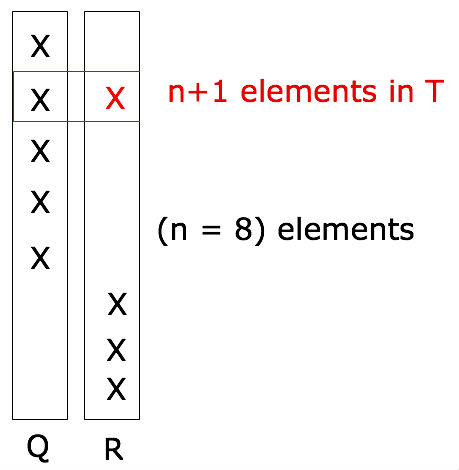
\includegraphics[scale=0.3]{Untitled.jpg}

\paragraph{
	Trying to map $T$, a subset of $S$, containing $n+1$ elements, to $n$ non matching elements is impossible, as illustrated through the \textit{Pigeon Hole Principle}. $T$ must match at least one element to it's corresponding number used to sum, as $n$ choices, with $n+1$ mapped values prevents us from creating a \textit{one-to-one} function from $T$ to the set of pairs in $S$. Therefore, it must be true that there exists two elements whose sum is $2n+1$.
}

\end{document}

%------------------------------------------------------------------------------
% End of journal.tex
%------------------------------------------------------------------------------
